\chapter{Multithreading}

\begin{summary}
Multithreading is a crucial concept in Java. It allows two or more parts of a program to be executed simultaneously to maximize CPU utilization. Video games, computer simulations, web servers, and browsers are examples of applications where the use of multithreading is essential. Various Java frameworks rely on multithreading. Therefore, it is important to understand the basic concepts.

Additionally, with the introduction of virtual threads as part of Project Loom, Java’s capability for handling concurrent operations is set to increase, allowing for a much larger number of threads to be managed with significantly less overhead. This is particularly beneficial for IO-bound and server-side applications.

Furthermore, mastering asynchronous programming techniques, such as those offered by CompletableFuture and Spring's asynchronous methods, enables developers to write non-blocking code that can perform tasks in the background, improving application responsiveness and overall throughput.
\end{summary}

\section{Introduction to Multithreading}

To fully grasp the term multithreading, we begin by explaining the difference between a thread and a process. A process is a program that is being executed. It can consist of one or more execution paths. These mini-processes within a program are called threads. Multithreading refers to writing a program in which multiple threads are implemented that can be executed simultaneously.

The different threads within a process can be executed at the same time, allowing the CPU to be utilized to its maximum potential. In a single-core CPU, there is a scheduler that decides which thread is executed and manages context switching between the different threads. This context switching happens so quickly that it seems as though multiple things are happening at once in the program. For example, imagine playing Pac-Man on a single-core CPU. The ghosts continuously move across the screen while you simultaneously input keyboard commands to control Pac-Man and dodge the ghosts.

In a multi-core CPU, the execution of different threads can genuinely occur simultaneously. However, a scheduler is still necessary to ensure that all threads get an equal share of processing time.

\begin{figure}[H]
  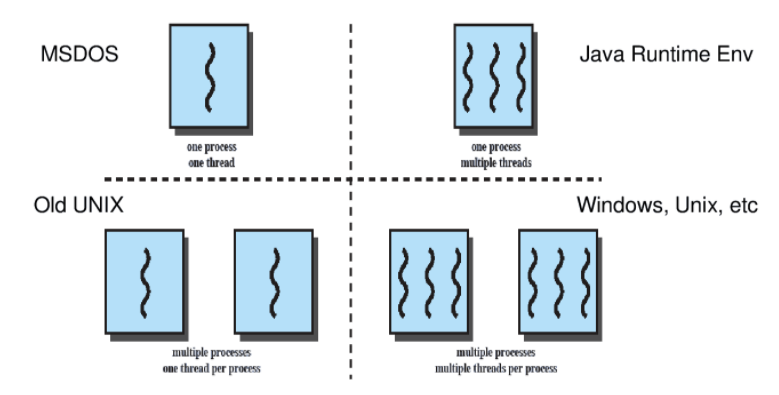
\includegraphics[width=\linewidth]{images/h9/process_threads.png} 
  \caption{Relatie tussen proces en threads}
  \label{fig:proces_thread}
\end{figure}

\begin{figure}[H]
  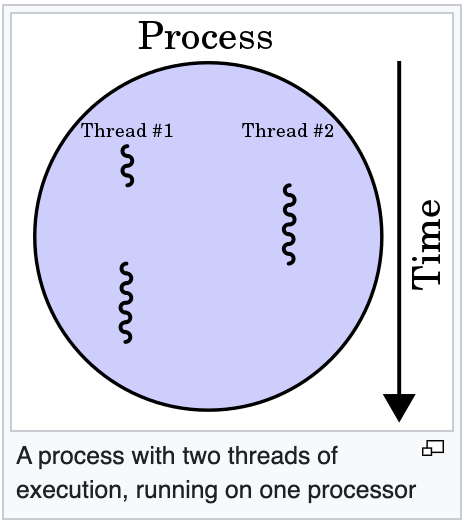
\includegraphics[scale=1]{images/h9/process_with_two_threads.png}
  \label{fig:proces_thread_2}
\end{figure}

Multitasking is the ability to perform more than one task at the same time. Java therefore provides thread-based multitasking. Within a process, threads share a portion of memory. This portion, known as the heap, is where the objects reside. Each thread also has a piece of private memory used during the execution of the thread, referred to as the stack. When the scheduler decides to activate another thread within a process, this context switch is carried out very efficiently.

\section{Use cases for multithreading}

Web Servers: In web servers, threads can handle multiple client requests simultaneously, improving the server's ability to serve more clients efficiently without waiting for each request to be processed sequentially.
Multimedia Applications: Applications that deal with multimedia processing, like video players or audio streaming services, use threads to ensure smooth playback while simultaneously downloading or buffering future content.
Financial Applications: In finance, real-time transaction processing systems use threads to handle high volumes of concurrent transactions, ensuring data consistency and quick response times during market hours.
Gaming: Modern video games use multithreading to separate logic and rendering processes, and to manage real-time user inputs along with game state management without lag.
Scientific Computing: Applications that perform complex simulations and data analysis can use threads to distribute the computational load across multiple CPU cores, significantly speeding up processing times.
Mobile Applications: Mobile apps often use threads to perform background tasks such as data synchronization, fetching updates, or performing lengthy computations while keeping the user interface responsive.

\section{Basics of Threads}

Threads are objects in Java. All Java programs have at least one thread, the main thread, which is created by the JVM (Java Virtual Machine) when the program is started. The main() method is executed by the main thread. In addition, you can create additional threads. You create these objects by either making a subclass of the Thread class or by implementing the functional interface Runnable. We will look at both possibilities.


\subsection{Creating Threads Using the Thread Class}

When you create a subclass of the Thread class, you override the run() method. The run() method contains the instructions that the thread will execute once you call the start() method.

\begin{lstlisting}
public class WorkerThread extends Thread {

	@Override
	public void run() {
		System.out.println("Line A (" + Thread.currentThread().getName() + ")");
		System.out.println("Line B (" + Thread.currentThread().getName() + ")");
		System.out.println("Line C (" + Thread.currentThread().getName() + ")");
		System.out.println("Line D (" + Thread.currentThread().getName() + ")");
		System.out.println("Line E (" + Thread.currentThread().getName() + ")");
	}

	public static void main(String[] args) {
		WorkerThread workerThread = new WorkerThread();
		workerThread.start();
		System.out.println("Line 1 (" + Thread.currentThread().getName() + ")");
		System.out.println("Line 2 (" + Thread.currentThread().getName() + ")");
		System.out.println("Line 3 (" + Thread.currentThread().getName() + ")");
	}
}
\end{lstlisting}


Once an instance of the WorkerThread class has been started, the scheduler alternates between the main thread and the WorkerThread instance. On a single-processor computer, it appears as though the threads are being executed simultaneously, while on a multi-processor computer, the threads can actually be executed at the same time.

Here is a possible sequence of the program:

\begin{verbatim}
Line A (Thread-0)
Line 1 (main)
Line B (Thread-0)
Line 2 (main)
Line C (Thread-0)
Line 3 (main)
Line D (Thread-0)
Line E (Thread-0)
\end{verbatim}


\subsection{Implementing the Runnable Interface}

A second way to program a thread is by creating a class that implements the java.lang.Runnable interface. Here as well, you must provide an implementation of the run() method. To start the thread, you need to pass an instance of the class that implements the Runnable interface as a parameter to a constructor of the Thread class. Then, you can call the start() method.

\begin{lstlisting}
public class WorkerThread2 implements Runnable {

	@Override
	public void run() {
		System.out.println("Line A (" + Thread.currentThread().getName() + ")");
		System.out.println("Line B (" + Thread.currentThread().getName() + ")");
		System.out.println("Line C (" + Thread.currentThread().getName() + ")");
		System.out.println("Line D (" + Thread.currentThread().getName() + ")");
		System.out.println("Line E (" + Thread.currentThread().getName() + ")");
	}

	public static void main(String[] args) {
		WorkerThread2 workerThread = new WorkerThread2();
		new Thread(workerThread).start();
		System.out.println("Line 1 (" + Thread.currentThread().getName() + ")");
		System.out.println("Line 2 (" + Thread.currentThread().getName() + ")");
		System.out.println("Line 3 (" + Thread.currentThread().getName() + ")");
	}
}
\end{lstlisting}

A common mistake is calling the run() method instead of the start() method. At first glance, this may not seem problematic. However, it does NOT result in a multithreaded program. Instead, the main thread will execute the instructions of the run() method. Test this out by calling run() instead of start() in the program above. Make sure you avoid this mistake!

\subsection{Runnable as a Lambda Expression}

Since the Runnable interface is a functional interface, you can also use a lambda expression to simplify your code. This approach is particularly useful for creating quick runnables without having to create a whole new class. Lambda expressions provide a concise way to implement the single abstract method of a functional interface.

Here is a simple example of using a lambda expression to implement Runnable:

\begin{lstlisting}
public class WorkerThread3 {

	public static void main(String[] args) {
		new Thread(() -> {
			System.out.println("Line A (" + Thread.currentThread().getName() + ")");
			System.out.println("Line B (" + Thread.currentThread().getName() + ")");
			System.out.println("Line C (" + Thread.currentThread().getName() + ")");
			System.out.println("Line D (" + Thread.currentThread().getName() + ")");
			System.out.println("Line E (" + Thread.currentThread().getName() + ")");
		}).start();
		System.out.println("Line 1 (" + Thread.currentThread().getName() + ")");
		System.out.println("Line 2 (" + Thread.currentThread().getName() + ")");
		System.out.println("Line 3 (" + Thread.currentThread().getName() + ")");
	}
}
\end{lstlisting}

In this example, the lambda expression () -> {...} implements the Runnable interface. It defines what the thread will do when executed, without the need for a separate Runnable class. This simplifies the code and makes it more readable, especially for short tasks or when working within a context where adding new classes would be cumbersome.


\subsection{Thread class versus Runnable Interface}

It may be a bit confusing that you have two possibilities for implementing threads. However, there are important differences between the two implementations. When you create a subclass of Thread, the objects of this class are 'real' thread objects and you, as a developer, have full control over the thread. When you use the Runnable interface, you are essentially only defining the work that needs to be performed by the thread. You then have no control over the thread itself.

If you make a subclass of the Thread class, you cannot use a second superclass because Java does not allow multiple inheritance. Therefore, if you want to inherit from another superclass, you use the Runnable interface.

\subsection{Virtual threads}

Real threads, or platform threads, in Java correspond directly to native OS threads. Each Java thread is a thin wrapper around these OS-level threads, which means they are managed and scheduled by the operating system. Real threads are powerful because they can run truly concurrently on multicore processors, leveraging parallelism. However, they also come with higher costs in terms of context switching, memory usage, and scheduling overhead, which can become significant when managing a large number of threads.

Virtual threads, introduced as part of Project Loom, aim to address the scalability issues posed by real threads. Unlike real threads, virtual threads are lightweight, managed entirely by the Java Virtual Machine (JVM) rather than the operating system. They are designed to have a low memory footprint and allow for massive concurrency. Virtual threads achieve this by decoupling the thread lifecycle from the underlying OS thread, using a scheduling technique known as 'fibers', which are scheduled by the JVM onto a smaller number of real threads.

\begin{lstlisting}
public class WorkerThread4 {

	public static void main(String[] args) {
		Thread virtualThread = Thread.startVirtualThread(() -> {
			System.out.println("Line A (" + Thread.currentThread().getName() + ")");
			System.out.println("Line B (" + Thread.currentThread().getName() + ")");
			System.out.println("Line C (" + Thread.currentThread().getName() + ")");
			System.out.println("Line D (" + Thread.currentThread().getName() + ")");
			System.out.println("Line E (" + Thread.currentThread().getName() + ")");
		});
		System.out.println("Line 1 (" + Thread.currentThread().getName() + ")");
		System.out.println("Line 2 (" + Thread.currentThread().getName() + ")");
		System.out.println("Line 3 (" + Thread.currentThread().getName() + ")");

        try {
            virtualThread.join(); // wait for the virtual thread to end
        } catch (InterruptedException e) {
            throw new RuntimeException(e);
        }
    }
}
\end{lstlisting}


\begin{lstlisting}
import java.util.concurrent.ExecutorService;
import java.util.concurrent.Executors;
import java.util.concurrent.ThreadFactory;
import java.util.concurrent.TimeUnit;

public class ThreadFactoryWithVirtualThread {

    public static void main(String[] args) {
        ThreadFactory virtualThreadFactory = Thread.ofVirtual().name("MyVirtualThread-", 0).factory();

        ExecutorService executor =
                Executors.newFixedThreadPool(4, virtualThreadFactory);

        for (int i = 0; i < 8; i++) {
            executor.submit(() -> {
                System.out.println("Running task in a virtual thread: "
                        + Thread.currentThread().getName());
            });
        }

        shutdownAndAwaitTermination(executor);
    }

    private static void shutdownAndAwaitTermination(ExecutorService executorService) {
        executorService.shutdown(); // Disable new tasks from being submitted
        try {
            // Wait a while for existing tasks to terminate
            if (!executorService.awaitTermination(10, TimeUnit.SECONDS)) {
                executorService.shutdownNow(); // Cancel currently executing tasks
                // Wait a while for tasks to respond to being cancelled
                if (!executorService.awaitTermination(10, TimeUnit.SECONDS)) {
                    System.err.println("Executor service failed to terminate.");
                }
            }
        } catch (InterruptedException ex) {
            executorService.shutdownNow();       // (Re-)Cancel if current thread also interrupted
            Thread.currentThread().interrupt();           // Preserve interrupt status
        }
    }
}
\end{lstlisting}

Here, we demonstrate the use of a ThreadFactory with virtual threads. We create a virtual thread factory using Thread.ofVirtual().factory(), and then use it to create a fixed-size thread pool with Executors.newFixedThreadPool(). Tasks submitted to this pool execute in virtual threads created by the virtual thread factory.

\begin{verbatim}
Running task in a virtual thread: MyVirtualThread-2
Running task in a virtual thread: MyVirtualThread-1
Running task in a virtual thread: MyVirtualThread-0
Running task in a virtual thread: MyVirtualThread-3
Running task in a virtual thread: MyVirtualThread-2
Running task in a virtual thread: MyVirtualThread-1
Running task in a virtual thread: MyVirtualThread-0
Running task in a virtual thread: MyVirtualThread-3
\end{verbatim}

\section{Thread life cycle}

A Java thread always has one of the following statuses:
\begin{itemize}
\item NEW\\
As soon as you create a Thread object, it has the status \textit{NEW}. As soon as the \textit{start()} method is called, the status of the thread changes from NEW to RUNNABLE.
\item RUNNABLE\\
A thread that is executed in the JVM (Java Virtual Machine) is in this status. There are 2 possibilities: either the thread is effectively being executed, or the thread is ready to be executed but is waiting for an available processor.
\item BLOCKED\\
A thread is in the BLOCKED status when the thread must wait to execute a synchronized code fragment. A synchronized code fragment is a method or part of a method that can only be executed by one thread at a time. If one thread is executing this code, other threads that want to start with this code fragment must wait. We will delve deeper into synchronization in this section.
\item WAITING\\
A thread is in the WAITING status if it is waiting for another thread that needs to perform a certain action first.
\item TIMED\_WAITING\\
A thread is in the status timed\_waiting just like in the waiting status if it is waiting for another thread to perform a certain action. The difference, however, is that the thread has a timeout set and will proceed after the preset time.
\item TERMINATED\\
A thread that has completed its task is in the status TERMINATED.
\end{itemize}

\begin{figure}[H]
  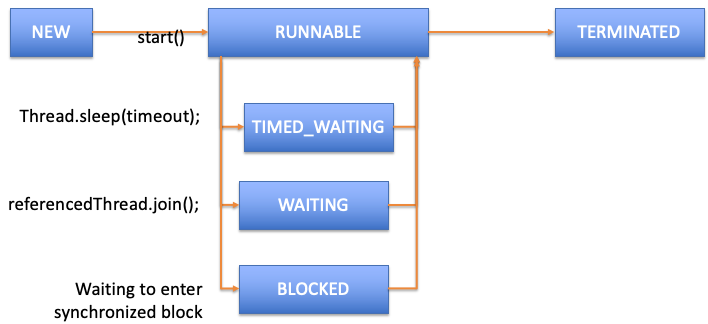
\includegraphics[width=\linewidth]{images/h9/thread_life_cycle.png}
  \label{fig:thread_life_cycle}
\end{figure}

\section{Common thread methods}


\subsection{Thread.sleep()}

The Thread.sleep() method can be used to pause a thread for a specified amount of time (expressed in milliseconds).
Note that this method is a static method.
When the Thread.sleep() instruction is executed, the thread scheduler will place the caller in WAIT status for the specified time. Once this time has passed, the thread's status becomes RUNNABLE again, and then it will have to wait until the CPU is available to continue execution. The actual time that the thread will thus 'sleep' is therefore dependent on the thread scheduler.

\begin{lstlisting}
public class WorkerThreadWithSleep extends Thread {

	@Override
	public void run() {
		System.out.println("Line A (" + Thread.currentThread().getName() + ")");
		try {
			Thread.sleep(5000);
		} catch (InterruptedException e) {
			e.printStackTrace();
		}
		System.out.println("Line B (" + Thread.currentThread().getName() + ")");
		System.out.println("Line C (" + Thread.currentThread().getName() + ")");
		System.out.println("Line D (" + Thread.currentThread().getName() + ")");
		System.out.println("Line E (" + Thread.currentThread().getName() + ")");
	}

	public static void main(String[] args) {
		WorkerThreadWithSleep workerThread = new WorkerThreadWithSleep();
		System.out.println(workerThread.getState());
		workerThread.start();
		System.out.println(workerThread.getState());
		System.out.println("Line 1 (" + Thread.currentThread().getName() + ")");
		System.out.println("Line 2 (" + Thread.currentThread().getName() + ")");
		System.out.println("Line 3 (" + Thread.currentThread().getName() + ")");
		System.out.println(workerThread.getState());
	}
}
\end{lstlisting}

After printing 'Line A...', the workThread goes to sleep for 5 seconds. The status of the workerThread then becomes TIMED\_WAITING, and the main thread can continue its activities. When the 5 seconds are up, the workThread can resume work.

\begin{oefening}
Create a class \textbf{Talker} that is a subclass of the class \textbf{java.util.Thread}.
You should include a property \textbf{id} (int) in this subclass and a constructor that allows you to create a Talker object and pass the id as a parameter.
When the thread is started, it will print its id 10 times, each time with a half-second pause.
Create 4 instances of the Talker class in the main program and start the threads.
\\
Then modify the Talker class so that it implements the Runnable interface. What changes do you need to make in your code?
\end{oefening}

\subsection{referencedThread.join()}

When a running thread calls the instruction referencedThread.join(), the executing thread enters the WAIT status. The thread remains waiting until the referencedThread is completely finished. If the referencedThread was already finished, the executing thread can simply continue with its tasks and does not need to wait, of course.


\begin{lstlisting}
public class WorkerThreadWithJoin extends Thread {

	@Override
	public void run() {
		System.out.println("Line A (" + Thread.currentThread().getName() + ")");
		System.out.println("Line B (" + Thread.currentThread().getName() + ")");
		System.out.println("Line C (" + Thread.currentThread().getName() + ")");
		System.out.println("Line D (" + Thread.currentThread().getName() + ")");
		System.out.println("Line E (" + Thread.currentThread().getName() + ")");
	}

	public static void main(String[] args) {
		WorkerThreadWithJoin workerThread = new WorkerThreadWithJoin();
		System.out.println(workerThread.getState());
		workerThread.start();
		System.out.println(workerThread.getState());
		System.out.println("Line 1 (" + Thread.currentThread().getName() + ")");
		try {
			workerThread.join();
		} catch (InterruptedException e) {
			e.printStackTrace();
		}
		System.out.println("Line 2 (" + Thread.currentThread().getName() + ")");
		System.out.println("Line 3 (" + Thread.currentThread().getName() + ")");
		System.out.println(workerThread.getState());
	}
}
\end{lstlisting}

After displaying 'Line 1...', the main thread will wait until the workerThread is completely finished. Only after the workerThread has concluded will the main thread resume execution. Therefore, the program will produce the following output.

\begin{verbatim}
NEW
RUNNABLE
Line 1 (main)
Line A (Thread-0)
Line B (Thread-0)
Line C (Thread-0)
Line D (Thread-0)
Line E (Thread-0)
Line 2 (main)
Line 3 (main)
TERMINATED
\end{verbatim}


\begin{oefening}
We are going to search for the integer between 1 and 10000 that has the greatest number of divisors. A divisor is a number that divides another without leaving a remainder. We want to know which number this is and how many divisors it has.

Create a class DivisorCounter. You can pass a minimum and maximum number to the constructor. This will be the range of numbers that the thread will test.
Initially, set these values to 1 and 10000. Write a method that can find the number with the highest number of divisors within this range. This method may be called directly from the constructor.
The found number (and the number of divisors) must be stored in a member variable.

Add a main() method that performs the calculation and prints the result.
The result should be either 7560 or 9240, as both numbers have 64 divisors.

Also, make sure you print the execution time of your calculation.

Try increasing the range to 50000 or 100000 numbers, and you will see that the execution time increases exponentially.

Modify your code so that you can divide the calculation into subproblems and have each part executed by a separate thread. Thus, you will make the DivisorCounter class a thread.
Then, in the main() method, write the necessary code to start several threads with a part of the range. Once the threads are done executing, finally make the necessary comparisons to determine which number has the greatest number of divisors from the entire range.

Check if your program now executes faster. With 10 threads, we get the following result:
\begin{verbatim}
Range [1-50000]
Getal: 45360
Aantal delers: 100
Tijd: 1.684 seconden
\end{verbatim}
\end{oefening}

\section{Thread synchronization}
Multithreading is a powerful technique, but it makes programs more difficult to control and debug, especially when threads start sharing resources.

In the following example, the shared resource is a cookie jar.
Here is the CookieBox class.

\begin{lstlisting}
public class CookieBox {

	private int numberOfCookies;

	public CookieBox(int numberOfCookies) {
		this.numberOfCookies = numberOfCookies;
	}

	public boolean takeCookie() {
			if (numberOfCookies > 0) {
				numberOfCookies--;
				return true;
			}
			return false;
	}
}
\end{lstlisting}

The class Child is a thread.

\begin{lstlisting}
public class Child extends Thread {

	private int numberOfCookies;
	private CookieBox cookieBox;
	private String name;

	public Child(String name, CookieBox cookieBox) {
		this.cookieBox = cookieBox;
		this.name = name;
	}

	@Override
	public void run() {
		while (cookieBox.takeCookie()) {
			numberOfCookies++;
			try {
				Thread.sleep(5);
			} catch (InterruptedException e) {
				e.printStackTrace();
			}
		}
		System.out.println(name + " had " + numberOfCookies + " cookies");
	}

	public int getNumberOfCookies() { return numberOfCookies; }
}
\end{lstlisting}

\begin{lstlisting}
public class EatingCookies {

	public static void main(String[] args) {
		CookieBox cookieBox = new CookieBox(50);
		Child[] children = { new Child("Bram", cookieBox),
				new Child("Sophie", cookieBox),
				new Child("Elke", cookieBox),
				new Child("Robin", cookieBox),
				new Child("Sammy", cookieBox),
				new Child("Max", cookieBox) };
        for (Child child : children) {
            child.start();
        }
        for (Child child : children) {
            try {
                child.join();
            } catch (InterruptedException e) {
                e.printStackTrace();
            }
        }
		System.out.println("Total amount of cookies: " +
				Arrays.stream(children)
						.mapToInt(Child::getNumberOfCookies)
						.sum());
	}
}
\end{lstlisting}

We create one CookieBox with 50 cookies and 6 Child threads that will all take cookies from this cookie jar. We start the 6 threads and pause the main() thread until all the Kind threads are finished and the cookie jar is empty. Then, we will ask the Kind threads how many cookies they have eaten.

\begin{verbatim}
Sammy had 10 cookies
Bram had 9 cookies
Sophie had 10 cookies
Elke had 9 cookies
Max had 10 cookies
Robin had 10 cookies
Total amount of cookies: 58
\end{verbatim}

Despite the fact that there are only 50 cookies in the cookie jar, the Child threads will still manage to eat a total of 58 cookies together. Clearly, something is going wrong.

\begin{figure}[H]
  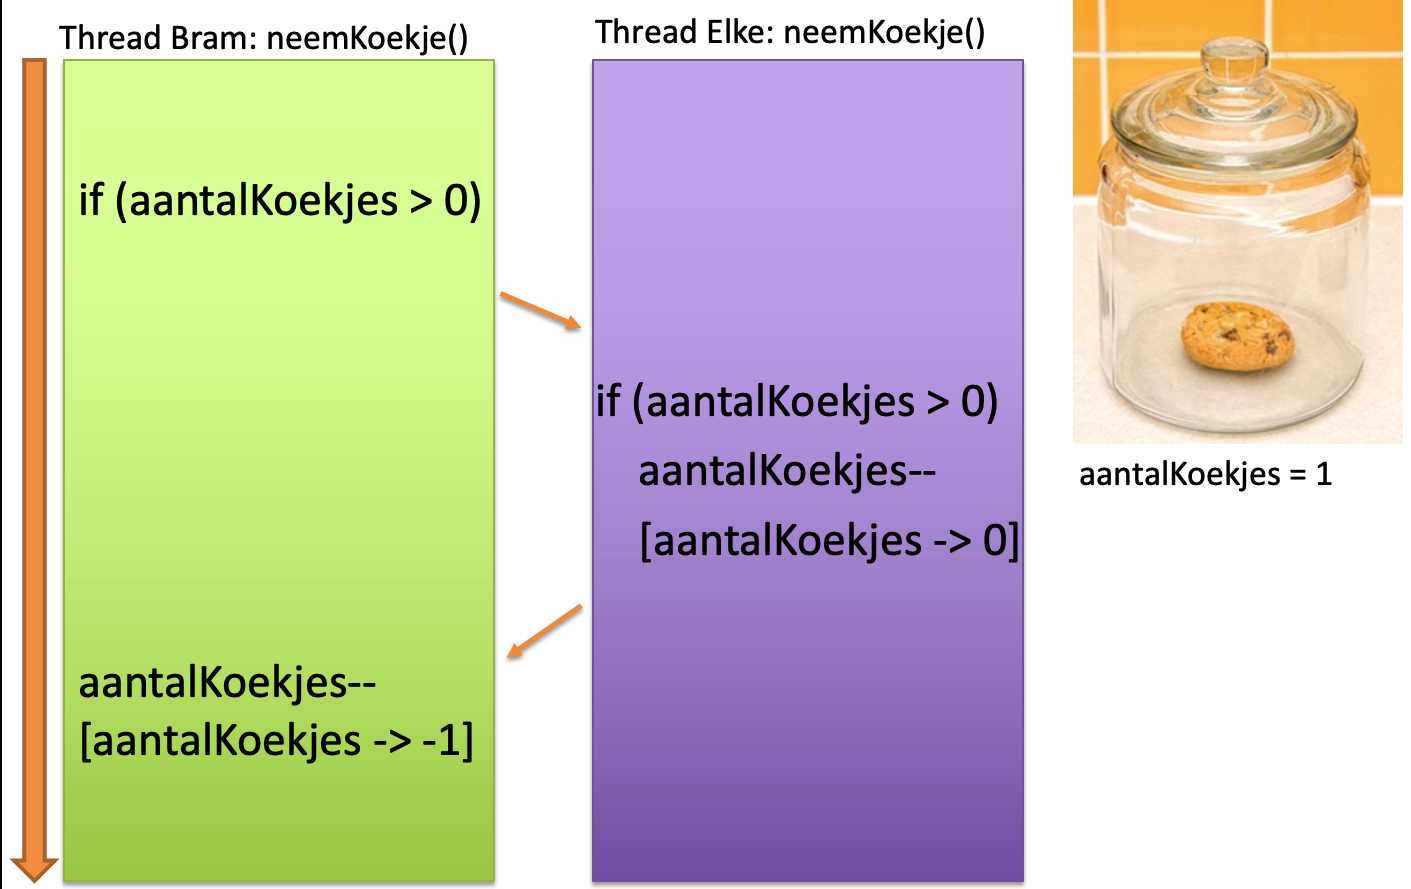
\includegraphics[width=\linewidth]{images/h9/koekjesdoos.png}
  \label{fig:concurrent_access}
\end{figure}

In the image above, we illustrate what goes wrong.
We assume that we have one processor and that there are two threads (Bram and Elke) executing the takeCookie() method simultaneously. There is still one cookie left in the cookie jar.
Thread Bram takes its turn and checks if there is a cookie available. This is the case, so the condition returns true. However, the thread scheduler decides it's Elke's turn. This thread checks if there is still a cookie and decreases the number of cookies by one. Now, it's Bram's turn again. The thread resumes its operations at the point of decreasing the number of cookies, and now we have -1 cookies.

The error occurred because thread Bram, after checking if there was still a cookie, did not immediately 'take' the cookie.
Therefore, the cookie jar needs to be secured in a way that another thread cannot intervene during the execution of the takeCookie() method.
Programmatically, we can solve this by marking the takeCookie() method with the \textbf{synchronized} keyword. This essentially places a lock on the Cookie Jar object, and if one thread is taking a cookie from the cookie jar, another thread cannot access the cookie jar. The other thread only gets access to the cookie jar once the previous thread has finished.

\begin{lstlisting}
public class CookieBox {

	private int numberOfCookies;

	public CookieBox(int numberOfCookies) {
		this.numberOfCookies = numberOfCookies;
	}

	public synchronized boolean takeCookie() {
			if (numberOfCookies > 0) {
				numberOfCookies--;
				return true;
			}
			return false;
	}
}
\end{lstlisting}

\subsection{Status WAITING, TIMED\_WAITING en BLOCKED}

\begin{lstlisting}
public class DemoStateBlocked extends Thread {

	private static int value = 0;
	private Thread parent;

	public DemoStateBlocked(Thread parent) {
		this.parent = parent;
	}

	@Override
	public void run() {
		commonResource();
		System.out.println(parent.getState());
	}

	private static synchronized void commonResource() {
		for (int i = 0; i < 100; i++) {
			value++;
			try {
				Thread.sleep(1);
			} catch (InterruptedException e) {
				e.printStackTrace();
			}
		}
		System.out.println(value);
	}

	public static void main(String[] args) throws InterruptedException {
		Thread t1 = new DemoStateBlocked(Thread.currentThread());
		Thread t2 = new DemoStateBlocked(Thread.currentThread());
		t1.start();
		t2.start();
		Thread.sleep(2);
		System.out.printf("%n%s - %s%n", t1.getState(), t2.getState());
		t2.join();
	}
}
\end{lstlisting}

The above program once again displays various thread statuses.
Observe what happens during the execution of the program and explain the statuses of the different threads.

\begin{verbatim}
TIMED_WAITING - BLOCKED
100
WAITING
200
WAITING
\end{verbatim}

What happens if the method commonResource() is not synchronized?

\section{Timer and TimerTask}

The class \textbf{java.util.TimerTask} is an abstract class that implements the Runnable interface. You can use this class if you want to execute a task at specific times.

In the run() method of a subclass or instance of the TimerTask class, you implement the actions of the task. In the instance repeatedTask in the example below, we show the start and end time of the task, and in between, there is a 2-second wait.

We use an object from the Timer class to schedule and start the task.
The Timer class contains various schedule() methods to execute a task on a given date or after a specified time (delay). There are also various methods named scheduleAtFixedRate() which allow you to repeat at a specified interval.

\begin{lstlisting}
import java.time.LocalDateTime;
import java.util.Timer;
import java.util.TimerTask;

public class RepeatTask {

	public static void main(String[] args) {
		TimerTask repeatedTask = new TimerTask() {
			public void run() {
				System.out.println("Task started on " + LocalDateTime.now());
				try {
					Thread.sleep(2000);
				} catch (InterruptedException e) {
					e.printStackTrace();
				}
				System.out.println("Task completed on " + LocalDateTime.now());
			}
		};
		Timer timer = new Timer("Timer");
		long period = 10000L;
		timer.scheduleAtFixedRate(repeatedTask, 0, period);
	}
}
\end{lstlisting}

Executing the program will give the following output:

\begin{verbatim}
Task started on 2020-12-14T14:50:42.207567
Task completed on 2020-12-14T14:50:44.207988
Task started on 2020-12-14T14:50:52.207359
Task completed on 2020-12-14T14:50:54.209605
\end{verbatim}

The task is started every 10 seconds (10,000 milliseconds) and will take approximately 2 seconds to execute.

When the execution time of the task is longer than the period between consecutive scheduled tasks, the tasks are placed in a queue, and the next task will start as soon as the previous task has finished. Test this out by adjusting the execution time and the period between consecutive tasks in the program RepeatTask.

You can use Timer and TimerTask in a Spring Boot application, but it's more common to use Spring's \textbf{@Scheduled} annotation for scheduling tasks. Both methods allow you to schedule tasks for future execution in a background thread, but they offer different levels of integration and flexibility, particularly in a Spring context.

\section{Concurrency framework}

\subsection{Concurrent collections}

A large number of Collection classes are not thread-safe. This means that they cannot be used concurrently by different threads without issues.
Concurrency control was not provided for the collections to maximize performance in a single-threaded program.

We illustrate the problem with an example. In the program below, we start 2 threads that both add 1000 numbers to a shared list. When both threads are finished, you would therefore expect there to be 2000 numbers in the list.

\begin{lstlisting}
import java.util.ArrayList;
import java.util.Collections;
import java.util.List;

public class ConcurrentCollection extends Thread {

	private int id;
	private List<Integer> numbers;

	public ConcurrentCollection(int id, List<Integer> myList) {
		this.id = id;
		this.numbers = myList;
	}

	@Override
	public void run() {
		for (int i =0; i < 1000; i++) {
			numbers.add(id + i);
		}
	}

	public static void main(String[] args) {
			List<Integer> values = new ArrayList<>();
			ConcurrentCollection t1 = new ConcurrentCollection(1000, values);
			ConcurrentCollection t2 = new ConcurrentCollection(10000, values);
			t1.start();
			t2.start();
			try {
				t1.join();
				t2.join();
			} catch (InterruptedException e) {
				e.printStackTrace();
			}

			System.out.println(values.size());

	}

}
\end{lstlisting}

When we run the program multiple times, we see the following numbers appear as output when we query the number of elements in the list.

\begin{verbatim}
1226
1551
1063
1598
2000
1837
1810
2000
2000
1620
\end{verbatim}

It is also possible that an exception occurs while running the program.
\begin{verbatim}
Exception in thread "Thread-4" java.lang.ArrayIndexOutOfBoundsException: Index 113 out of bounds for length 109
	at java.base/java.util.ArrayList.add(ArrayList.java:486)
	at java.base/java.util.ArrayList.add(ArrayList.java:498)
	at be.pxl.multithreading.collections.ConcurrentCollection.run(ConcurrentCollection.java:20)
\end{verbatim}

The problem is solved by making the ArrayList a synchronizedList.

\begin{lstlisting}
List<Integer> values = Collections.synchronizedList(new ArrayList<>());
\end{lstlisting}

\subsubsection{Producer-consumer problem}

A classic synchronization problem is the producer-consumer problem (also known as the bounded-buffer problem). In the producer-consumer problem, we have two threads: the producer and the consumer, who both share a common buffer of a fixed size. The producer's task is to generate data and place it in the buffer. At the same time, the consumer processes the data that appears on the buffer. When the buffer is full, the producer must wait before placing new data on the buffer. When the buffer is empty, the consumer must wait until new data is produced.
In the literature, you will find several other classic synchronization problems (such as the dining philosophers) and problems that can be caused by synchronization (such as deadlocks), but these are beyond the scope of this course.

\subsection{Atomic variables}

The AtomicInteger and other atomic classes in Java are part of the java.util.concurrent.atomic package. These classes provide a way to perform atomic (i.e., thread-safe without using synchronization) operations on single variables. Essentially, they offer a non-blocking mechanism to perform thread-safe operations on single values, which can be significantly faster than using synchronized blocks.
 
\begin{lstlisting}
import java.util.concurrent.atomic.AtomicInteger;

public class CookieBox {

	private AtomicInteger numberOfCookies;

	public CookieBox(int numberOfCookies) {
		this.numberOfCookies = new AtomicInteger(numberOfCookies);
	}

	public boolean takeCookie() {
		int result = numberOfCookies.getAndDecrement();
		return result > 0;
	}
}
\end{lstlisting}


\subsection{ExecutorService framework}

The ExecutorService framework is an API that makes a whole group (pool) of threads available, to which you can assign tasks.

There are several factory methods available to create an ExecutorService object. The following line of code shows how you can create a thread pool with 10 threads:

\begin{lstlisting}
ExecutorService executor = Executors.newFixedThreadPool(10);
\end{lstlisting}

Now you can assign a task to the ExecutorService. The ExecutorService can handle two types of tasks: Runnable and Callable tasks. Callable is an enhanced version of Runnable that was added since Java 1.5.

Callable$<$V$>$ is a generic functional interface with a method call() that returns a value of the generic datatype V as a result.

\begin{lstlisting}
import java.util.Random;
import java.util.concurrent.Callable;
import java.util.concurrent.ExecutorService;
import java.util.concurrent.Executors;
import java.util.concurrent.Future;

public class GeneratingFutureString {

	public static void main(String[] args) {
		ExecutorService executorService = Executors.newFixedThreadPool(5);

		Callable<String> generateRandomLetters = () -> {
			int leftLimit = 'a'; // letter 'a'
			int rightLimit = 'z'; // letter 'z'
			int targetStringLength = 10;
			Random random = new Random();
			StringBuilder buffer = new StringBuilder(targetStringLength);
			for (int i = 0; i < targetStringLength; i++) {
				int randomLimitedInt = leftLimit + (int) (random.nextFloat() * (rightLimit - leftLimit + 1));
				buffer.append((char) randomLimitedInt);
				try {
					Thread.sleep(1000);
				} catch (InterruptedException e) {
					e.printStackTrace();
				}
			}
			return buffer.toString();
		};
		Future<String> result = executorService.submit(generateRandomLetters);


		System.out.println("Counting down...");
		for (int i = 10; i >= 0; i--) {
			System.out.println(i);
		}
		if (result.isDone()) {
			System.out.println("generating letters is done.");
		} else {
			System.out.println("generating letters is running.");
		}
		executorService.shutdown();
	}

}
\end{lstlisting}

\subsubsection{CompletableFuture}

CompletableFuture is a class introduced in Java 8 that allows us to write asynchronous, non-blocking code. It is a powerful tool that can help us write code that is more efficient and responsive.

\begin{lstlisting}
CompletableFuture<String> future = CompletableFuture.supplyAsync(() -> {
    try {
        Thread.sleep(5000);
    } catch (InterruptedException e) {
        e.printStackTrace();
    }
    return "Hello, world!";
});

future.thenAccept(result -> System.out.println(result));
\end{lstlisting}


\section{Parallel streams}

Parallelism is the concept where a problem is divided into several subproblems. You can then assign different threads to work on solving each subproblem. Ultimately, the solution is obtained by combining the solutions of the subproblems.

It is possible to execute streams serially or in parallel. Here is the Employee class.

\begin{lstlisting}
public class Employee {
	private String name;
	private int salary;

	public Employee(String name, int salary) {
		this.name = name;
		this.salary = salary;
	}

	public int getSalary() {
		return salary;
	}
}
\end{lstlisting}

You now want to know how many employees have a salary of 15,000 or more. This can also be calculated in parallel. With the IntStream class, you must use the parallel() method, while with collections, you use parallelStream().

\begin{lstlisting}
public class ParallellStreams {

	public static void main(String[] args) {
		List<Employee> employees = new ArrayList<>();
		for (int i = 0; i < 100; i++) {
			employees.add(new Employee("A", 20000));
			employees.add(new Employee("B", 3000));
			employees.add(new Employee("C", 15002));
			employees.add(new Employee("D", 7856));
			employees.add(new Employee("E", 200));
			employees.add(new Employee("F", 50000));
		}
		long t1 = System.currentTimeMillis();

		System.out.println("Sequential Stream Count?= " +
				employees.stream().filter(e -> e.getSalary() >= 15000).count());

		long t2 = System.currentTimeMillis();
		System.out.println("Sequential Stream Time Taken?= " + (t2 - t1) + "\n");
		t1 = System.currentTimeMillis();

		System.out.println("Parallel Stream Count?= " +
				employees.parallelStream().filter(e -> e.getSalary() >= 15000).count());

		t2 = System.currentTimeMillis();
		System.out.println("Parallel Stream Time Taken?= " + (t2 - t1));
	}
}
\end{lstlisting}


\begin{verbatim}
Sequential Stream Count?= 300
Sequential Stream Time Taken?= 19

Parallel Stream Count?= 300
Parallel Stream Time Taken?= 8
\end{verbatim}

\section{Exercises}

\begin{oefening}
\textbf{Simulation of the use of a bank account}\
The following program settings are managed via properties (program properties):
\begin{itemize}
\item Starting balance for a bank account
\item Number of users who have access to the bank account
\item Number of transactions that each user will carry out (each user will perform an equal number of transactions)
\item Limit value for a transaction (both for withdrawals and deposits)
\end{itemize}

Now create a bank account with the specified starting balance.\\
Create a thread for each user that will perform the specified number of transactions, which can be either withdrawals or deposits. Take into account the specified limit value. Note that the balance of the bank account should never become negative.\\
Each transaction, along with the result of the transaction, is written in a transaction log file.
\end{oefening}

\begin{oefening}
\textbf{Producer-Consumer}\\
This application simulates a production line where multiple threads simultaneously and at different rates place new products. Another thread processes the products on the line at a certain speed. The application can be used to test whether the processing unit can handle the speed.
 
\begin{figure}[H]
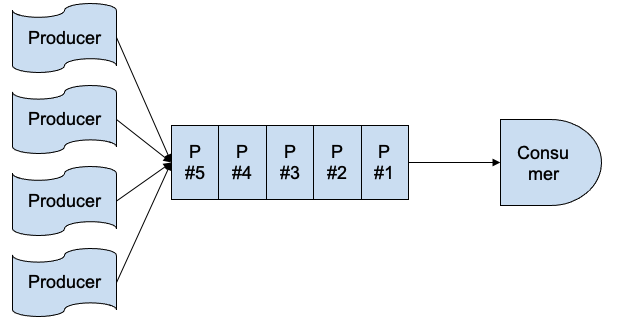
\includegraphics[width=\linewidth]{images/h9/opgave_producer_consumer.png}
\caption{Producers en consumer}
\label{fig:producer_consumer}
\end{figure}

\textbf{Package}\\
The Package class is already provided; it contains only a constructor that assigns an ID or sequence number to each new package on the line and also provides a toString method. A class variable is used for this, so this value does not need to be provided when creating a Package.
\\
\textbf{ProductionLine}\\
Create a ProductionLine class that will represent the production line. On the production line, you can only add new products at the end and take them from the front. Use a collection of your choice from the Collection framework. Provide methods to add a Package to the end of the production line (addPackage()) and to take a Package from the front (getPackage()). Remember to remove the taken packages from the production line.
Ensure that no exceptions can occur if there are no packages left on the line.
Make sure that all operations on the production line are synchronized, so it is not possible for multiple threads to perform an operation on the collection at the same time. (For this, you only need to make adjustments to the addPackage() and getPackage() methods of the ProductionLine class).
\\
\textbf{Producer}\\
Create the Producer class. This will create new Packages at a steady pace and add them to the production line. The Producer must be able to run as a thread, so provide the necessary for that. In the constructor, you must provide two parameters: the rate at which new products are created and the production line object. The rate is the number of packages this producer creates per minute.
When the Producer thread is started, it must continuously create new Packages and add them to the production line, with a pause in between to maintain the specified rate (use Thread.sleep(milliseconds) for this). The thread gives a short notification in the console each time a new package is placed on the line.
The correct number of milliseconds the Producer should wait between two packages can be calculated as follows: (60 / rate) * 1000
\\
\textbf{Consumer}\\
The Consumer class is similar: it must also be able to run as a thread, and the constructor also includes the rate (= again the number of packages that the Consumer can process per minute) and the production line object.
Upon starting, the Consumer will continuously take packages from the production line (always from the front) at the specified rate. Use the method you have provided for this in the ProductionLine class.
The thread prints out each package processed. Also, when no packages are available on the production line, this is reported via a message in the console.
\\
\textbf{Main Method}\\
Finally, provide a main method. Use this to create 4 Producers with rates of 20, 15, 12, and 7. Then also create a Consumer with a rate of 30. The Consumer thus processes 30 packages per minute and works faster than the 4 Producers.
Make sure all these components are correctly started and work in parallel. This way, you should be able to analyze whether the Consumer works fast enough to handle the 4 simultaneous Producers.
\end{oefening}
